%%%%%%%%%%%%%%%%%%%%%%%%%%%%%%%%%%%%%%%%%%%%%%%%%%%%%%%%%%%%%%%%%%%%%%%%%%%%%%%%%%%%%%%%%%%%%%%%%%%%%%%%%%%
\documentclass[conference]{IEEEtran}
\usepackage{cite}
\usepackage{amsmath,amssymb,amsfonts}
\usepackage{algorithmic}
\usepackage{graphicx}
\usepackage{textcomp}
\usepackage{listings}
\usepackage{xcolor}
\usepackage{pgfplots}
\usepackage{geometry}
\usepackage{array}
\usepackage{placeins}
\def\BibTeX{{\rm B\kern-.05em{\sc i\kern-.025em b}\kern-.08em
    T\kern-.1667em\lower.7ex\hbox{E}\kern-.125emX}}

% Define colors for code highlighting

\definecolor{backcolour}{rgb}{0.9,0.9,0.9}
\definecolor{plotblack}{rgb}{0,0,0}
\definecolor{plotgray}{rgb}{0.6,0.6,0.6}
% Define listing style
\lstdefinestyle{mystyle}{
    backgroundcolor=\color{backcolour},
    basicstyle=\ttfamily\footnotesize,
    breakatwhitespace=false,
    breaklines=true,
    captionpos=b,
    keepspaces=true,
    numbers=right,
    numbersep=-5 pt,
    showspaces=false,
    showstringspaces=false,
    showtabs=false,
    tabsize=2
}
\lstset{style=mystyle}

\begin{document}
%%%%%%%%%%%%%%%%%%%%%%%%%%%%%%%%%%%%%%%%%%%%%%%%%%%%%%%%%%%%%%%%%%%%%%%%%%%%%%%%%%%%%%%%%%%%%%%%%%%%%%%%%%%
\title{A Comparative Analysis of Ray and Dask: Scaling Frameworks for Big Data Analysis and Machine Learning in Python\\
}
%%%%%%%%%%%%%%%%%%%%%%%%%%%%%%%%%%%%%%%%%%%%%%%%%%%%%%%%%%%%%%%%%%%%%%%%%%%%%%%%%%%%%%%%%%%%%%%%%%%%%%%%%%%
\author{\IEEEauthorblockN{Athanasios Varis}
\IEEEauthorblockA{\textit{ECE} \\
\textit{NTUA}\\
Athens, Greece \\
el19606@mail.ntua.gr}
\and
\IEEEauthorblockN{Giorgos Vlachopoulos}
\IEEEauthorblockA{\textit{ECE} \\
\textit{NTUA}\\
Athens, Greece \\
el19926@mail.ntua.gr}
\and
\IEEEauthorblockN{Ioannis Nikiforidis}
\IEEEauthorblockA{\textit{ECE} \\
\textit{NTUA}\\
Athens, Greece \\
el18123@mail.ntua.gr}
}
%%%%%%%%%%%%%%%%%%%%%%%%%%%%%%%%%%%%%%%%%%%%%%%%%%%%%%%%%%%%%%%%%%%%%%%%%%%%%%%%%%%%%%%%%%%%%%%%%%%%%%%%%%%
\maketitle
%%%%%%%%%%%%%%%%%%%%%%%%%%%%%%%%%%%%%%%%%%%%%%%%%%%%%%%%%%%%%%%%%%%%%%%%%%%%%%%%%%%%%%%%%%%%%%%%%%%%%%%%%%%
\begin{abstract}
As the volume and complexity of data continue to surge, the demand for efficient and scalable frameworks for big data analysis and machine learning has become crucial. This paper provides a comparative analysis of Ray and Dask, two Python-based frameworks designed to address the challenges of distributed computing in large-scale data and machine learning applications. The study delves into the  features and performance characteristics of both Ray and Dask, exploring their capabilities in handling distributed computing tasks, parallelizing computations, and seamlessly scaling across clusters. We examine their suitability for various use cases. Through bench-marking experiments and real-world use cases, this paper aims to provide insights into the strengths and limitations of Ray and Dask, aiding practitioners and researchers in selecting the most appropriate framework based on their specific requirements. The findings contribute to a deeper understanding of the trade-offs involved in choosing between these two scaling frameworks, ultimately guiding decision-making processes in the context of big data analysis and machine learning tasks in Python.
\end{abstract}
%%%%%%%%%%%%%%%%%%%%%%%%%%%%%%%%%%%%%%%%%%%%%%%%%%%%%%%%%%%%%%%%%%%%%%%%%%%%%%%%%%%%%%%%%%%%%%%%%%%%%%%%%%%
\begin{IEEEkeywords}
python, scaling frameworks, ray, dask, big data analysis, machine learning
\end{IEEEkeywords}
%%%%%%%%%%%%%%%%%%%%%%%%%%%%%%%%%%%%%%%%%%%%%%%%%%%%%%%%%%%%%%%%%%%%%%%%%%%%%%%%%%%%%%%%%%%%%%%%%%%%%%%%%%%
\section{System and Software Description}
\subsection{Virtual Machines\cite{b1,b2}}
In this project we will be using Virtual Machines provided by Okeanos-Knossos to conduct our experiments. Virtual Machines provide flexibility, efficiency and scalability.
\begin{itemize}
\item \textbf{Isolation:} Virtual machines provide a level of isolation between different applications and services running on the same physical hardware. This isolation enhances security by minimizing the risk of one application affecting or compromising another.
\item \textbf{Consistent Environments:} VMs enable the creation of consistent and reproducible environments across different stages of a project's life-cycle. This helps in avoiding compatibility issues between development, testing, and production environments, ensuring a smoother deployment process.
\item \textbf{Resource Efficiency:} VMs allow for efficient resource utilization by enabling multiple virtualized instances to run on a single physical server.
\item \textbf{Scalability:} Virtual machines facilitate scalability by allowing you to dynamically adjust resources allocated to each VM based on changing project requirements. This adaptability ensures that your project can scale up or down efficiently to handle varying workloads.
\item \textbf{Cost Savings:} Using virtual machines can lead to cost savings by reducing the need for physical hardware and associated maintenance costs. It allows for better utilization of existing hardware and provides a more cost-effective solution.
\end{itemize}
\subsection{Python\cite{b3,b4}}
Python has become a powerhouse in the fields of big data analysis and machine learning, owing to its versatility, extensive libraries, and a vibrant community of developers. Here are a few key aspects of big data analysis and machine learning in Python:
\begin{itemize}
\item \textbf{Extensive Libraries:} Python boasts a rich ecosystem of libraries specifically designed for big data analytics and machine learning. Libraries such as NumPy, pandas, and scikit-learn provide robust tools for data manipulation, analysis, and machine learning model development.
\item \textbf{Scalability with Dask and Ray:} Frameworks like Dask and Ray empower Python developers to scale their applications seamlessly. These tools enable parallel and distributed computing, allowing users to process large datasets and execute machine learning tasks efficiently across clusters of machines.
\item \textbf{Machine Learning Frameworks:} Python is home to some of the most widely used machine learning frameworks, including TensorFlow and PyTorch. These frameworks facilitate the development, training, and deployment of complex machine learning models, covering a broad spectrum of applications from computer vision to natural language processing.
\item \textbf{Data Visualization:} Python excels in data visualization, with libraries like Matplotlib, Seaborn, and Plotly offering powerful tools for creating insightful visualizations. Effective data visualization is crucial for understanding complex patterns and trends in big datasets.
\item \textbf{Community Support:} Python's large and active community plays a vital role in the development and adoption of tools for big data analysis and machine learning. This community-driven approach results in frequent updates, extensive documentation, and a wealth of tutorials and resources.
\item \textbf{Interoperability:} Python integrates well with other technologies and languages, making it a preferred choice for building end-to-end data pipelines. It can seamlessly connect with databases, cloud services, and other programming languages, allowing for smooth transitions between different stages of data processing and analysis.
\item \textbf{Education and Accessibility:} Python's syntax is clear and concise, making it an accessible language for beginners. This has contributed to its popularity in educational settings and has led to a growing pool of data scientists and engineers with proficiency in Python.
\end{itemize}
In summary, Python's versatility, extensive library support, scalability through frameworks like Dask and Ray, and a thriving community make it a go-to language for big data analysis and machine learning applications. Its ecosystem empowers developers and data scientists to tackle complex problems, analyze vast datasets, and build sophisticated machine learning models with ease.

\subsection{Ray\cite{b5,b6}}
Ray is a distributed computing framework for Python that is designed to make it easy to scale and parallelize applications. Ray provides a simple API for parallel and distributed computing, allowing developers to write scalable applications without needing to explicitly manage the complexities of distributed systems. Key features of Ray include:
\begin{itemize}
\item \textbf{Task Parallelism:} Ray allows you to parallelize Python functions, turning them into distributed tasks that can run in parallel across a cluster of machines.
\item \textbf{Distributed Data Processing:} Ray provides abstractions for working with distributed data, making it easier to scale data processing tasks.
\item \textbf{Distributed Memory:} Ray supports distributed memory, allowing you to share data between tasks running on different machines.
\item \textbf{Actor Model:} Ray extends the actor model, providing a way to create distributed stateful objects that can encapsulate both data and computation.
\item \textbf{Ray Libraries:} Ray includes libraries that leverage its capabilities for specific use cases, such as RLlib for reinforcement learning and Tune for hyperparameter tuning.
\item \textbf{Dynamic Task Graphs:} Ray dynamically constructs task dependency graphs, enabling efficient scheduling of tasks and resource management.
\end{itemize}
Ray is commonly used in the fields of machine learning, distributed computing, and reinforcement learning. It provides a flexible and scalable solution for parallel and distributed computing tasks, making it easier for developers to build applications that can scale across large clusters of machines.

\subsection{Dask\cite{b7,b8}}
Dask is another distributed computing framework for Python, but it focuses on parallel computing and task scheduling. It's particularly well-suited for parallelizing operations on large data-sets that don't fit into memory. Key features of Dask include:
\begin{itemize}
\item \textbf{Dynamic Task Scheduling:} Dask breaks down large computations into smaller tasks and dynamically schedules them to run in parallel. This allows for the efficient use of resources and can handle computations that are larger than the available memory.
\item \textbf{Parallel Data Structures:} Dask provides parallel versions of familiar data structures in Python, such as arrays (Dask Arrays), dataframes (Dask DataFrames), and bags (Dask Bags). These structures can scale computations beyond the limits of a single machine.
\item \textbf{Integration with Existing Libraries:} Dask integrates seamlessly with popular Python libraries such as NumPy, pandas, and scikit-learn, allowing users to parallelize and distribute their existing code without significant modifications.
\item \textbf{Support for Out-of-Core Computing:} Dask can handle datasets that are larger than available memory by intelligently loading and unloading data from disk as needed.
\item \textbf{Scalability:} Dask can scale from a laptop to a cluster of machines, making it suitable for a wide range of computing environments.
\end{itemize}
Dask is commonly used in data science and machine learning workflows where large datasets need to be processed, analyzed, or transformed efficiently. It provides a user-friendly interface for parallel and distributed computing in Python, making it easier for data scientists and researchers to scale their computations.
%%%%%%%%%%%%%%%%%%%%%%%%%%%%%%%%%%%%%%%%%%%%%%%%%%%%%%%%%%%%%%%%%%%%%%%%%%%%%%%%%%%%%%%%%%%%%%%%%%%%%%%%%%%
\section{Installation and Setup}
\subsection{Prerequisites}
To perform this project, we developed three virtual machines in order to extensively examine parallel data processing. In the first virtual machine we acted as the master while the second and the third ones acted as a workers. For the operating system, we chose Ubuntu 16.04.3 LTS and configured 4 cores, 8 gigabytes of RAM, and 30 gigabytes of hard disk space for each virtual machine. We then configured the installation environment, including Python and the Ray and Dask working frameworks.
\subsection{Ubuntu}
First we need to upgrade the linux environment. So we execute the following throught the terminal :
\begin{lstlisting}[language=bash]
sudo apt update
sudo apt upgrade
\end{lstlisting}
\subsection{Python}
In order to setup Python enter the following to a terminal :
\begin{lstlisting}[language=bash]
sudo apt install python3
python3 --version
\end{lstlisting}
The final line is to make sure that the python environment is set-up correctly. Now since pip will be used in order to install the frameworks, the following step is needed as well :
\begin{lstlisting}[language=bash]
sudo apt install python3-pip
\end{lstlisting}
Also, since Dask uses 'numpy', installing it is mandatory and can be gone with the following line :
\begin{lstlisting}[language=bash]
python3 -m pip install -U numpy
\end{lstlisting}
And 'numpy' uses 'sciPy' thus :
\begin{lstlisting}[language=bash]
python3 -m pip install -U sciPy
\end{lstlisting}
To aid with some machine learning applications we use 'scikit-learn' and 'lightgbm'
\begin{lstlisting}[language=bash]
python3 -m pip install -U scikit-learn
python3 -m pip install -U lightgbm
\end{lstlisting}
Finally, in order to distribute workloads the package 'python-distributed' is needed and can be installed by :
\begin{lstlisting}[language=bash]
sudo apt install python-distributed
\end{lstlisting}
\subsection{Ray}
After making sure that Python has been installed correctly, the following can be entered to the terminal in order to install the Ray framework.
\begin{lstlisting}[language=bash]
python3 -m pip install -U ray[default]
\end{lstlisting}
\subsection{Dask}
Finally, the Dask framework is installed.
\begin{lstlisting}[language=bash]
python3 -m pip install -U dask[complete]
\end{lstlisting}
\subsection{Networking}
In order for the distribution of tasks to take place, there needs to be a connection between the machines. In real world scenarios in data centers, the machines are typically connected by Ethernet, through network switches and hubs that segment and provide hierarchy and organisation to the whole center. In this case, since the machines are virtual, they are placed in the same NAT network and given public ipv6 addresses so they can communicate with each other and still retain the ability to be connected to the internet. Since the data utilized and produced by this project are not high risk or sensitive, there is no need for extra security measures, but ideally the worker machines should be blocked from accessing or be accessed from public addresses so a potential attacker has fewer access points.
%%%%%%%%%%%%%%%%%%%%%%%%%%%%%%%%%%%%%%%%%%%%%%%%%%%%%%%%%%%%%%%%%%%%%%%%%%%%%%%%%%%%%%%%%%%%%%%%%%%%%%%%%%%
\section{Subjects of Analysis}

\subsection{Classification\cite{b9}}
Classification stands as a cornerstone in supervised machine learning, where the primary objective is to train a model using labeled data. This trained model then goes on to predict the class labels of previously unseen instances. The essence lies in deciphering a mapping from input features to predetermined output classes, empowering the model to provide accurate predictions for new data points. In the realm of large-scale data environments, the strategic distribution of classification tasks among multiple machines emerges as a pivotal strategy for achieving scalability and efficiency. In essence, the distributed workload approach is instrumental in handling the computational demands of expansive datasets that may overwhelm the capabilities of a single machine. By harnessing the collective power of multiple machines, we can significantly accelerate the training process, parallelizing computations and reducing the overall time required. This distributed paradigm not only addresses the challenges posed by big data but also optimizes resource utilization, ensuring that each machine contributes meaningfully to the classification process.

\subsection{Grid Search\cite{b10}}
Grid search is a hyperparameter tuning technique widely used in machine learning to systematically explore a predefined set of hyperparameter combinations for a given model. It involves training and evaluating the model with each combination, helping identify the optimal set of hyperparameters that yield the best performance on a validation set.While grid search is indeed a potent tool for model optimization, its practical application in the context of big data introduces additional complexities, necessitating thoughtful considerations. The strategic distribution of workloads emerges as a pivotal factor in enhancing its efficiency within the landscape of large-scale datasets.This involves not only dealing with the sheer scale of the datasets but also capitalizing on parallelization to streamline the hyperparameter optimization journey. Deliberate attention to nuances such as data distribution, optimal resource utilization, and streamlined communication becomes indispensable when seamlessly integrating distributed grid search into the fabric of big data environments.

\subsection{Clustering\cite{b11}}
Clustering, a fundamental unsupervised machine learning technique, plays a pivotal role in data analysis by uncovering inherent structures within datasets. The process involves grouping similar data points into clusters, providing insights into patterns and relationships without relying on predefined labels. Common clustering algorithms, including K-means, hierarchical clustering, and DBSCAN, offer versatile solutions tailored to diverse datasets.In the realm of big data, where datasets are vast and dimensionalities are high, challenges arise in the scalability and computational efficiency of clustering algorithms. Pairing clustering algorithms with distributed computing frameworks empowers data scientists and analysts to efficiently analyze vast datasets, uncover meaningful patterns, and gain valuable insights. This combination aligns with the demands of modern data analytics, where the volume and complexity of data necessitate scalable and parallelized solutions for effective clustering.

\subsection{Principal Component Analysis\cite{b12}}
Principal Component Analysis (PCA) is a dimensionality reduction technique commonly used in machine learning and data analysis to transform high-dimensional datasets into a lower-dimensional space while retaining as much variance as possible. The primary goal of PCA is to identify the principal components, which are linear combinations of the original features, that capture the most significant variability in the data. In the context of distributed computing, performing PCA on large-scale datasets poses challenges related to computational efficiency and scalability. Distributed frameworks such as Ray and Dask provide solutions to address these challenges and enable the application of PCA on big data.
%%%%%%%%%%%%%%%%%%%%%%%%%%%%%%%%%%%%%%%%%%%%%%%%%%%%%%%%%%%%%%%%%%%%%%%%%%%%%%%%%%%%%%%%%%%%%%%%%%%%%%%%%%%
\section{Data generation and Database loading}
We decided to create our own data through a Python script, with the aim of achieving better control and more immediate availability. This data, although generated through random number selection, has been parameterized to reflect realistic datasets. This approach allows the data to be used as naturally generated data sets, thus providing a realistic representation of the environments where the project will be implemented. This approach to data generation seeks to enhance the usability and accuracy of the results, while enhancing the flexibility and control of the experiment.

\subsection{Dataset for Classification and Grid Search}
We generated a data file that contained synthetic classification data and saved it in the LIBSVM format. The python function that generates it accepts as input 3 variables, which are the number of samples (number of data points) , the number of features (number of features per data point) and the number of classes (number of classes or labels). Since we could be dealing with data-sets that are larger than the usable RAM of the system, the data can be generated in smaller segments (chunks) which will later be concatenated in a singular file. A small file containing the metadata of the data file is also generated to provide an overview of the file. The following settings were used to produce our desired datasets based on the size we wanted to achieve :
 \begin{table}[ht]
    \centering
    \begin{tabular}{|c|c|c|}
    \hline
    ~ & 1GB & 2GB\\
    \hline
    Samples & 5 M & 10 M\\
    \hline
    Features & 10 & 10\\
    \hline
    \end{tabular}
\end{table}
\subsection{Dataset for Clustering and PCA}
We used a function to generate synthetic data resembling a Swiss roll and saved it in a file in the LIBSVM format. The parameters of the function are the number of samples (number of data points) and the noise ( the standard deviation of the Gaussian noise added to the data). We solve the problem of generating larger than RAM data by dividing the generation into chunks that fit into memory and the concatenate them in a single file. A small file containing the metadata of the data file is also generated to provide an overview of the file.The following settings were used to produce our desired datasets based on the size we wanted to achieve :
 \begin{table}[ht]
    \centering
    \begin{tabular}{|c|c|c|}
    \hline
    ~ & 1GB & 2GB\\
    \hline
    Samples & 15 M & 25 M\\
    \hline
    Noise & 0.2 & 0.2\\
    \hline
    K-Means & 16 & clusters \\
    \hline
    \end{tabular}
\end{table}

%%%%%%%%%%%%%%%%%%%%%%%%%%%%%%%%%%%%%%%%%%%%%%%%%%%%%%%%%%%%%%%%%%%%%%%%%%%%%%%%%%%%%%%%%%%%%%%%%%%%%%%%%%%
\section{Setting up the clusters}

\subsection{Ray}
\subsubsection{Master}
After having successfully set up the Ray framework, we can proceed to the terminal of the virtual machine we have assigned as the master, and enter the following:
\begin{lstlisting}[language=bash]
ray start --head
\end{lstlisting}
This will start the ray head node and provide us with the url of the ray dashboard.
\subsubsection{Workers}
After having successfully set up the Ray framework, and the scheduler is already running we can proceed to the terminal of the virtual machines we have assigned as the workers, and enter the following:
\begin{lstlisting}[language=bash]
ray start --address <IP>:6379
\end{lstlisting}
This will start a Ray worker process that will connect to the IP provided (in our case the IP that was given to the Master virtual machine).
\subsection{Dask}
\subsubsection{Master}
After having successfully set up the Dask framework, we can proceed to the terminal of the virtual machine we have assigned as the master, and enter the following:
\begin{lstlisting}[language=bash]
dask scheduler
\end{lstlisting}
This will start the scheduler and assign an IP address to it. In addition to the IP address, two ports will also be assigned to it, which by default are 8786 for the scheduler and 8787 for the dashboard.
\subsubsection{Workers}
After having successfully set up the Dask framework, and the scheduler is already running we can proceed to the terminal of the virtual machines we have assigned as the workers, and enter the following:
\begin{lstlisting}[language=bash]
dask worker tcp://<IP>:8786
\end{lstlisting}
This way, we create a worker that will automatically connect to the scheduler, given that the IP address and port we provided are correct. We can have greater control while creating a worker, and specify how much memory it has access to and how many threads it is allowed to use, with the following parameters :
\begin{lstlisting}[language=bash]
--nthreads 1 --memory-limit 1GB
\end{lstlisting}
%%%%%%%%%%%%%%%%%%%%%%%%%%%%%%%%%%%%%%%%%%%%%%%%%%%%%%%%%%%%%%%%%%%%%%%%%%%%%%%%%%%%%%%%%%%%%%%%%%%%%%%%%%%
\section{Code for measuring performance}
Since Ray and Dask are scaling frameworks, they do not affect the majority of the python code we want to execute. Apart from the different methods to connect to the clusters, there are some notable differences in some small parts of the code.
\subsection{Notable code differences}
\subsubsection{Data handling and loading}
\begin{itemize}
    \item \textit{Ray :} Data is loaded from .libsvm file into a numpy array. 
\end{itemize}
\begin{itemize}
    \item \textit{Dask :} Data is loaded from .libsvm file into a Dask dataframe which is then converted into a Dask array.
\end{itemize}
\subsubsection{Classification}  
\begin{itemize}
    \item \textit{Ray :} Our data is loaded into a numpy array, then a configuration space for hyperparameter tuning is setup and finally the tuning is done using Ray Tune.
\end{itemize}
\begin{itemize}
    \item \textit{Dask :} Our data is loaded into a dask dataframe and then converted to a dask array and finally Dask-ML's train\_test\_split is used to perform the train-test split step to help evaluate each classifier .
\end{itemize}
\subsubsection{Grid Search}
\begin{itemize}
\item \textit{Ray :} We use ray.tune.grid\_search to perform grid search.
\end{itemize}
\begin{itemize}
\item \textit{Dask :} In order to perform grid search we use dask\_ml.model\_selection.GridSearchCV using cross-validation.
\end{itemize}
\subsubsection{Clustering}
\begin{itemize}
    \item \textit{Ray :} Ray does not provide any specific APIs for clustering so we use the tools provided by sklearn.cluster
\end{itemize}

\begin{itemize}
    \item \textit{Dask :} Dask has dask\_ml.cluster that provides us with unsupervides clustering algorithms, such as KMeans.
\end{itemize}

\subsubsection{PCA}
\begin{itemize}
    \item \textit{Ray :} We use PCA from sklearn.decomposition to perform principal component analysis.
\end{itemize}

\begin{itemize}
    \item \textit{Dask :} The Dask framework provides us with dask\_ml.decomposition.PCA to perform principal component analysis.
\end{itemize}

\subsection{Connecting to the clusters}
\subsubsection{Ray}
In the beginning of the file that contains the python code we want to execute, we need to add the following :
\begin{lstlisting}[language=python]
ray.init(address="<IP>:6379")
\end{lstlisting}
Now, the process that is responsible for running the python script will connect to the Ray cluster to distribute the tasks. Between the brackets is the IP address of the machine where the master node is running. At the end of the file we add :
\begin{lstlisting}[language=python]
ray.shutdown()
\end{lstlisting}
To close the connection to the head node.
\subsubsection{Dask}
In the beginning of the file that contains the python code we want to execute, we need to add the following :
\begin{lstlisting}[language=python]
client = Client("tcp://<IP>:8786")
\end{lstlisting}
Now, the process that is responsible for running the python script will connect to the Dask cluster to distribute the tasks. Between the brackets is the IP address of the machine where the scheduler is running. At the end of the file we add :
\begin{lstlisting}[language=python]
client.close()
\end{lstlisting}
To close the connection to the scheduler, so it can be used for another process.
%%%%%%%%%%%%%%%%%%%%%%%%%%%%%%%%%%%%%%%%%%%%%%%%%%%%%%%%%%%%%%%%%%%%%%%%%%%%%%%%%%%%%%%%%%%%%%%%%%%%%%%%%%%
\FloatBarrier
\section{Results}
Initially, our project aimed to assess the performance of large datasets. However, constraints imposed by hardware limitations and unforeseen bugs hindered our ability to test datasets of 3, 7, and 10 gigabytes, as originally intended. Despite our best efforts, we restricted our evaluations to smaller datasets of 1GB and 2GB. Consequently, our study focused on comparing the efficiency and accuracy of the Ray and Dask frameworks in handling these reduced dataset sizes.
\subsection{Classification}
\FloatBarrier
    \begin{figure}
    \centering
    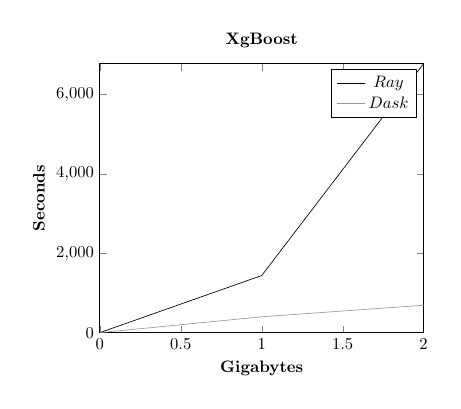
\begin{tikzpicture}[scale=0.6]
    \begin{axis}[
    xlabel={$\textbf{Gigabytes}$},
    ylabel={$\textbf{Seconds}$},
    title={\textbf{$\textbf{XgBoost}$}},
    xmin=0, xmax=2, % Set x-axis limits
    ymin=0, ymax=6780, % Set y-axis limits
    ]
    \addplot[plotblack] coordinates {
    (0, 0)
    (1, 1440)
    (2, 6780)
    };
    \addplot[plotgray] coordinates {
    (0, 0)
    (1, 400)
    (2, 690)
    };
    \legend{$Ray$, $Dask$}
    \end{axis}
    \end{tikzpicture}
    \caption{XgBoost - Time to complete computations.}
    \end{figure}
    \begin{table}
    \centering
    \scalebox{0.85}{
    \begin{tabular}{|c|c|c|}
    \hline
    \multicolumn{3}{|c|}{Time}\\
    \hline
    ~ & 1GB & 2GB\\
    \hline
    Ray & 1470 & 6780\\
    \hline
    Dask & 400 & 990\\
    \hline
    \multicolumn{3}{|c|}{Accuracy}\\
    \hline
    ~ & 1GB & 2GB\\
    \hline
    Ray & 0.70 & 0.87\\
    \hline
    Dask & 0.70 & 0.69\\
    \hline
    \end{tabular}}
    \caption{XgBoost Time and Accuracy.}
    \end{table}
    \begin{figure}
    \centering
    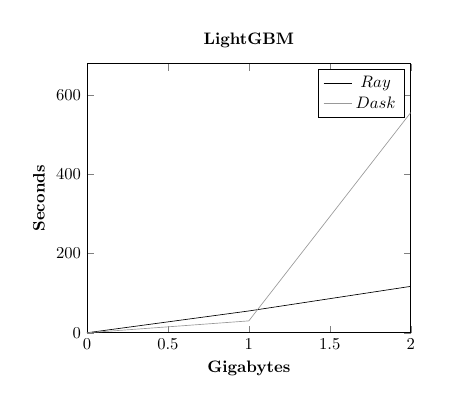
\begin{tikzpicture}[scale=0.6]
    \begin{axis}[
    xlabel={$\textbf{Gigabytes}$},
    ylabel={$\textbf{Seconds}$},
    title={\textbf{$\textbf{LightGBM}$}},
    xmin=0, xmax=2, % Set x-axis limits
    ymin=0, ymax=678, % Set y-axis limits
    ]
    \addplot[plotblack] coordinates {
    (0, 0)
    (1, 55)
    (2, 117)
    };
    \addplot[plotgray] coordinates {
    (0, 0)
    (1, 30)
    (2, 555)
    };
    \legend{$Ray$, $Dask$}
    \end{axis}
    \end{tikzpicture}
    \caption{LightGBM - Time to complete computations.}
    \end{figure}
    \begin{table}
    \centering
    \scalebox{0.85}{
    \begin{tabular}{|c|c|c|}
    \hline
    \multicolumn{3}{|c|}{Time}\\
    \hline
    ~ & 1GB & 2GB\\
    \hline
    Ray & 55 & 117\\
    \hline
    Dask & 30 & 555\\
    \hline
    \multicolumn{3}{|c|}{Accuracy}\\
    \hline
    ~ & 1GB & 2GB\\
    \hline
    Ray & 0.85 & 0.79\\
    \hline
    Dask & 0.33 & 0.40\\
    \hline
    \end{tabular}}
    \caption{LightGBM Time and Accuracy.}
    \end{table}
\FloatBarrier
    \begin{figure}[ht]
    \centering
    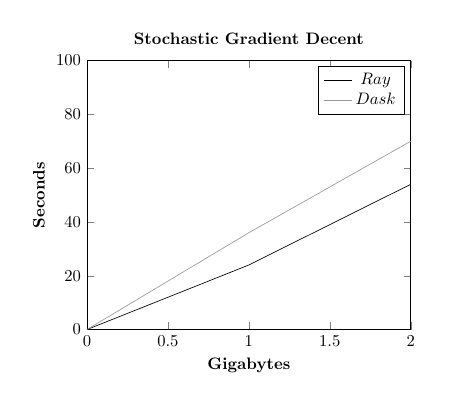
\begin{tikzpicture}[scale=0.6]
    \begin{axis}[
    xlabel={$\textbf{Gigabytes}$},
    ylabel={$\textbf{Seconds}$},
    title={\textbf{$\textbf{Stochastic Gradient Decent}$}},
    xmin=0, xmax=2, % Set x-axis limits
    ymin=0, ymax=100, % Set y-axis limits
    ]
    \addplot[plotblack] coordinates {
    (0, 0)
    (1, 24)
    (2, 54)
    };
    \addplot[plotgray] coordinates {
    (0, 0)
    (1, 36)
    (2, 70)
    };
    \legend{$Ray$, $Dask$}
    \end{axis}
    \end{tikzpicture}
    \caption{SGD - Time to complete computations.}
    \end{figure}
    \begin{table}[h]
    \centering
    \scalebox{0.85}{
    \begin{tabular}{|c|c|c|}
    \hline
    \multicolumn{3}{|c|}{Time}\\
    \hline
    ~ & 1GB & 2GB\\
    \hline
    Ray & 24 & 54\\
    \hline
    Dask & 36 & 70\\
    \hline
    \multicolumn{3}{|c|}{Accuracy}\\
    \hline
    ~ & 1GB & 2GB\\
    \hline
    Ray & 0.60 & 0.55\\
    \hline
    Dask & 0.60 & 0.55\\
    \hline
    \end{tabular}}
    \caption{SGD Time and Accuracy.}
    \end{table}
    \begin{figure}[h]
    \centering
    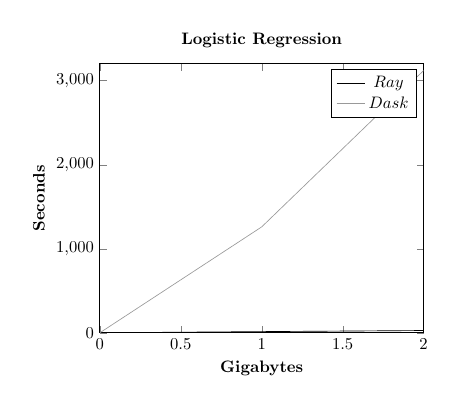
\begin{tikzpicture}[scale=0.6]
    \begin{axis}[
    xlabel={$\textbf{Gigabytes}$},
    ylabel={$\textbf{Seconds}$},
    title={\textbf{$\textbf{Logistic Regression}$}},
    xmin=0, xmax=2, % Set x-axis limits
    ymin=0, ymax=3200, % Set y-axis limits
    ]
    \addplot[plotblack] coordinates {
    (0, 0)
    (1, 14)
    (2, 27)
    };
    \addplot[plotgray] coordinates {
    (0, 0)
    (1, 1260)
    (2, 3120)
    };
    \legend{$Ray$, $Dask$}
    \end{axis}
    \end{tikzpicture}
    \caption{LR - Time to complete computations.}
    \end{figure}
    \begin{table}[h!]
    \centering
    \scalebox{0.85}{
    \begin{tabular}{|c|c|c|}
    \hline
    \multicolumn{3}{|c|}{Time}\\
    \hline
    GB/Sec & 1GB & 2GB\\
    \hline
    Ray & 14 & 27\\
    \hline
    Dask & 1260 & 3120\\
    \hline
    \multicolumn{3}{|c|}{Accuracy}\\
    \hline
    GB/Ac & 1GB & 2GB\\
    \hline
    Ray & 0.60 & 0.55\\
    \hline
    Dask & 0.58 & 0.55\\
    \hline
    \end{tabular}}
    \caption{LR Time and Accuracy.}
    \end{table}
    

\subsection{Clustering}
    \begin{figure}[h]
    \centering
    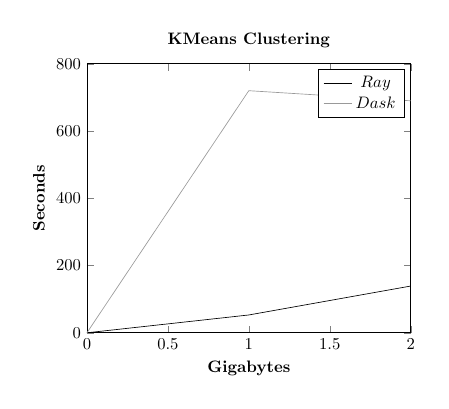
\begin{tikzpicture}[scale=0.6]
    \begin{axis}[
    xlabel={$\textbf{Gigabytes}$},
    ylabel={$\textbf{Seconds}$},
    title={\textbf{$\textbf{KMeans Clustering}$}},
    xmin=0, xmax=2, % Set x-axis limits
    ymin=0, ymax=800, % Set y-axis limits
    ]
    \addplot[plotblack] coordinates {
    (0, 0)
    (1, 53)
    (2, 139)
    };
    \addplot[plotgray] coordinates {
    (0, 0)
    (1, 720)
    (2, 690)
    };
    \legend{$Ray$, $Dask$}
    \end{axis}
    \end{tikzpicture}
    \caption{Clustering - Time to complete computations.}
    \end{figure}
    \begin{table}[ht]
    \centering
    \scalebox{0.85}{
    \begin{tabular}{|c|c|c|}
    \hline
    \multicolumn{3}{|c|}{Time}\\
    \hline
    GB/Sec & 1GB & 2GB\\
    \hline
    Ray & 53 & 139\\
    \hline
    Dask & 720 & 690\\
    \hline
    \multicolumn{3}{|c|}{Davis-Bouldin Score}\\
    \hline
    GB/Sc & 1GB & 2GB\\
    \hline
    Ray & 1.05 & 1.01\\
    \hline
    Dask & 0.77 & 0.75\\
    \hline
    \end{tabular}}
    \caption{Clustering Time and DB Score.}
    \end{table}
\FloatBarrier
%%%%%%%%%%%%%%%%%%%%%%%%%%%%%%%%%%%%%%%%%%%%%%%%%%%%%%%%%%%%%%%%%%%%%%%%%%%%%%%%%%%%%%%%%%%%%%%%%%%%%%%%%%%
\section{Observations}
\subsection{Classification}
\subsubsection{XgBoost}
Concerning XGBoost, Ray emerges as the more accurate framework, albeit with a slower runtime. Notably, as the dataset size grows, the computational time required by Ray increases significantly more than that of Dask. XgBoost also seems to require the most ammount of time out of any other computation we performed.
\subsubsection{LightGBM}
LightGBM demonstrates a moderate performance in terms of running speed. Intriguingly, while Ray maintains a higher level of accuracy, Dask exhibits a notable slowdown, particularly with larger dataset sizes.
\subsubsection{SGD}
In SGD, we observe comparable performance and scaling with data size across both frameworks. Notably, Ray exhibits a slight speed advantage, while both frameworks maintain an equivalent level of accuracy.
\subsubsection{LR}
In the case of Logistic Regression (LR), despite similar accuracy levels, the efficiency of Dask is notably worse.
\subsection{Clustering}
In Clustering, Ray exhibits superior performance with smaller datasets, whereas Dask's effectiveness appears to improve as datasets expand. Our evaluation, employing the Davies-Bouldin score, consistently reveals that Dask maintains lower scores, indicating superior performance.
%%%%%%%%%%%%%%%%%%%%%%%%%%%%%%%%%%%%%%%%%%%%%%%%%%%%%%%%%%%%%%%%%%%%%%%%%%%%%%%%%%%%%%%%%%%%%%%%%%%%%%%%%%%
\section{Conclusion}
Ray and Dask are versatile frameworks, boasting ease of application and scalability. While each excels in different tasks, our findings underscore substantial variations in efficiency even when performing similar operations. The choice between Ray and Dask hinges on the specific use case. Comprehensive research, conducted on more robust hardware and well-established datasets, would provide a deeper understanding.

Dask demonstrates straightforwardness in comparison to Ray, proving simpler to set up and operate. In summary, given the considerable variability in results, users and developers are advised to assess their intended operations and conduct thorough testing with both frameworks to determine the optimal choice. Notably, due to Dask's optimization for handling larger-than-memory datasets, it is expected to outperform in scenarios involving such datasets.
%%%%%%%%%%%%%%%%%%%%%%%%%%%%%%%%%%%%%%%%%%%%%%%%%%%%%%%%%%%%%%%%%%%%%%%%%%%%%%%%%%%%%%%%%%%%%%%%%%%%%%%%%%%
\begin{thebibliography}{00}
\bibitem{b1} "Home | okeanos-knossos IAAS ." https://okeanos-knossos.grnet.gr/home
\bibitem{b2} "What is a virtual machine (VM)?." https://www.redhat.com/en/topics/virtualization/what-is-a-virtual-machine
\bibitem{b3} "Welcome to Python.org." https://www.python.org
\bibitem{b4} "Our Success Stories | Python.org. " https://www.python.org/success-stories
\bibitem{b5} "Productionizing and scaling Python ML workloads simply | Ray." https://www.ray.io
\bibitem{b6} "Ray Documentation." https://docs.ray.io/en/latest/index.html
\bibitem{b7} "Dask | Scale the Python tools you love." https://www.dask.org
\bibitem{b8} "Dask Documentation." https://docs.dask.org/en/stable
\bibitem{b9} "What is Data Classification and Why is it Important?" https://www.techtarget.com/searchdatamanagement/definition/data-classification
\bibitem{b10} "Grid Search for model tuning." https://towardsdatascience.com/grid-search-for-model-tuning-3319b259367e
\bibitem{b11} "Clustering in Machine Learning." https://www.javatpoint.com/clustering-in-machine-learning
\bibitem{b12} "Principal Component Analysis (PCA) Explained." https://builtin.com/data-science/step-step-explanation-principal-component-analysis
\end{thebibliography}
%%%%%%%%%%%%%%%%%%%%%%%%%%%%%%%%%%%%%%%%%%%%%%%%%%%%%%%%%%%%%%%%%%%%%%%%%%%%%%%%%%%%%%%%%%%%%%%%%%%%%%%%%%%
\end{document}
%%%%%%%%%%%%%%%%%%%%%%%%%%%%%%%%%%%%%%%%%%%%%%%%%%%%%%%%%%%%%%%%%%%%%%%%%%%%%%%%%%%%%%%%%%%%%%%%%%%%%%%%%%%